\section{Development and testing}

\subsection{Hardware assembly}

\subsection{Programming the hardware}

\subsection{Range tests}

One of the most important tests to carry out prior to deployment in the field
was testing the range of the devices.

In this experiment I took four challenger RP2040s to The Downs, a large public
park in Bristol. Here I tested four different antenna configurations to compare
how well the signal travelled across an increasing distance. Signal strength can
be measured using the received signal strength index (RSSI), a measure of the
difference in signal from the transmitter to the receiver and measured in
decibels (CHECK THIS).

For the test, two challengers were programmed as transmitters, sending an
example data packet similar to the data that would eventually be used at the
farm. One of the transmitters used a simple PCB antenna
(Figure~\ref{fig:pcb-antenna}) while the other used a higher range whip style
antenna (Figure~\ref{fig:good-antenna}). Then I programmed two challengers as
receivers, again one had a low range antenna and the other a long range one.

This meant that four different antenna configurations could be tested
concurrently, as the receivers could pick up the signal from each transmitter.
An estimate of their estimated relative performance before testing is shown
below:

\begin{enumerate}
    \item Whip antenna to whip antenna (Likely best result)
    \item PCB antenna to whip antenna
    \item Whip antenna to PCB antenna
    \item PCB antenna to PCB antenna (Likely poorest result)
\end{enumerate}

The reason PCB transmitter to whip receiver will likely outperform the whip to
PCB configuration is that generally it is more important that the receiver has
better "hearing" capabilities than the transmitter can "shout".

Nine different distances from transmitter to receiver were tested, in 200m
increments starting from 0m as a baseline to a distance of 1600m
(Figure~\ref{fig:range-test-markers}). An important aspect in getting a
successful LoRa connection is whether there is line of sight between the
transmitter and receiver. Figure~\ref{fig:range-test-elevation} shows the
elevation profile of the test area, with the initial large dip being an
inaccuracy from google earth's topology data as the 0m point is near a cliff
edge. The lowest elevation point is at the starting point at around 83m above
sea level, while the highest point was at the 1km mark at around 94m making an
elevation range of 11m. My hypothesis was that signal would likely drop off or
stop entirely beyond this point as points beyond 1000m would be below the hill
line. This would effectively mean that the receivers would be in a signal shadow
point where the transmission waves would not be able to reach them. The only
possibility for signal to reach this area would be from reflections either from
nearby buildings or topology. However the effects of reflections are virtually
impossible to account for in the real world and therefore no accurate
predictions could be made.

\begin{figure}[H]
    \centering
    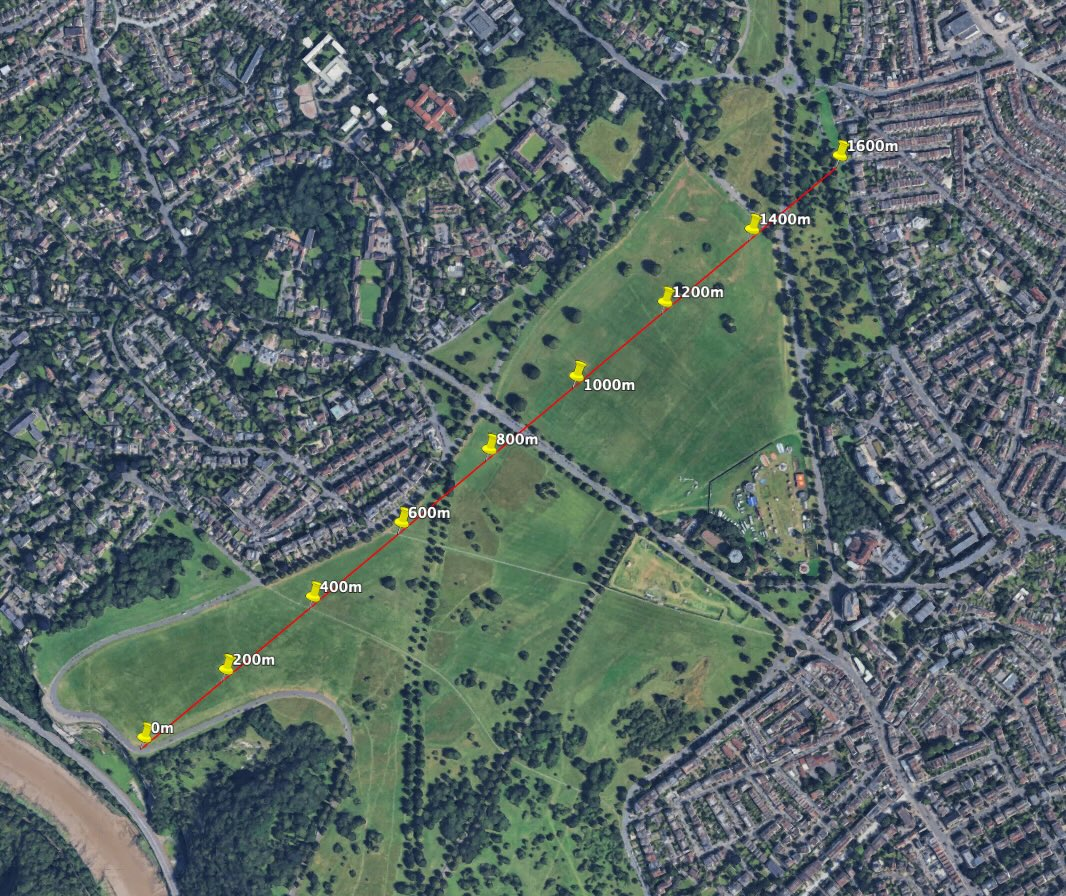
\includegraphics[width=0.8\textwidth]{contents/23-hw-development/23-fig/range-test-markers.jpg}
    \caption{Google earth image of data collection points}
    \label{fig:range-test-markers}
\end{figure}


\begin{figure}[H]
    \centering
    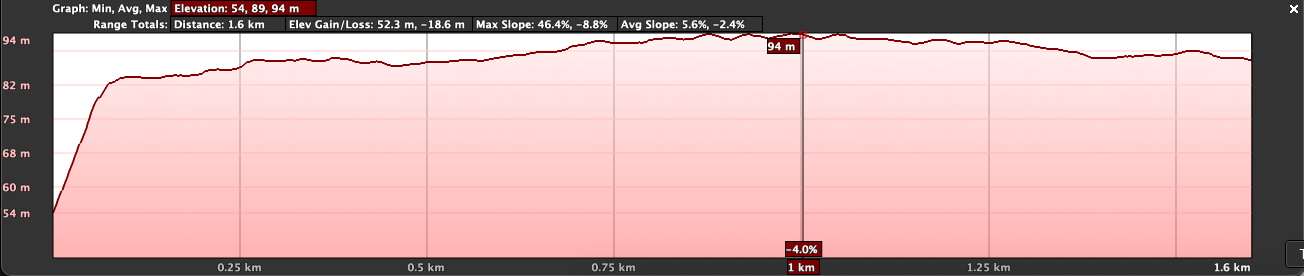
\includegraphics[width=1\textwidth]{contents/23-hw-development/23-fig/range-test-elevation-profile.jpg}
    \caption{Elevation profile of test area (ignore large dip at start)}
    \label{fig:range-test-elevation}
\end{figure}

At the time of the actual test however a festival was being run between the
1200m and 1400m mark. The festival had a number of large tents and temporary
buildings constructed which almost certainly blocked the signal. Therefore tests
past this point should be heavily caveated. It is likely this contributed to the
lack of signal past this point. Final data below (ADD DATA)

\subsection{Battery tests}

There is no mains electricity available in the apple field so the nodes must be
able to operate without external power source. Even with the use of a solar
panel the node must be able to work through the night and during periods of
dense cloud coverage where the solar panel will not have sufficient power to
keep the node running. This is where the use of a battery is particularly useful
as the solar panel can charge the battery with excess energy during periods of
excess solar radiation, such as during midday hours, and then store this energy
for periods of low or no solar radiation.

However, while daylight will be of little concern during the summer months when
this dissertation is being written, there will be far fewer days of usable
sunlight over the winter period. As the UK has very high latitude, there is
large seasonal variation in the length of a day. For the town of crediton
(nearest town to \farmName), in the summer there are 16.5 hours of daylight
while in winter it receives only 7.6 hours; meaning a night that is 16.4 hours
long. Therefore the node must have a battery sufficiently large to power it for
a minimum of 16.4 hours with some additional charge to account for high cloud
cover during the early evening and morning period.

To see if the battery solution was sufficient for this environment a test
was run on a fully charged 18650 battery that was then connected to the solar
power manager to allow the voltage to be regulated up to the challenger's 5v
input voltage. The node was then run with it's software and full suite of
sensors attached.

The node was then ran until the battery would no longer discharge, with the
final battery life of the node being 19 hours and 17 minutes.

A digital multimeter was installed between the solar power manager and the
challenger's usb c input to view the voltage and current in real time as well as
running a timer for the test and a calculation of the number of watt-hours
consumed by the node. During the test the node used 80ma at 5V for a wattage of
0.4W. The meter showed that the node consumed 7.96Wh of power. Considering the
battery capacity is 9 Wh it may seem that the battery ran out too quickly.
However, the solar power manager documentation tells us that the battery boost
efficiency - being the conversion of battery voltage from native 3.7V to 5V
output - is only 86\%.

With that in mind effective battery capacity is roughly 7.74Wh, which is very
similar to the actual result.

\subsection{Solar testing}

